\section{Architecture of the new system}
  System architecture is described by Ian Sommerville as:
  \begin{quote}
    \textit{'Software architecture is the fundamental organization of a system embodied in its
    components, their relationships to each other and to the environment, and the principles
    guiding its design and evolution.'} [1]
  \end{quote}

  Following will be the proposed design for ACME and a discussion on programming languages and how they relate to design decisions made. 
  Details of the design can be found in \hyperref[sec:AppendixB]{\textbf{Appendix B}}.

  \subsection{Overall Architecture}
  The architecture I have chosen is a Cloud-Native architecture. AWS, the largest cloud provider [2], describes this architecture as the 
  \textit{'approach of building, deploying, and managing modern applications in cloud computing environments'} [3]. In simpler terms, these are 
  servers for customers to use, but housed by AWS. These servers use virtualisation \textit{'allows the hardware elements of a single computer ... 
  to be divided into multiple virtual computers'} [4]. 

  \begin{figure}[H]
    \centering
    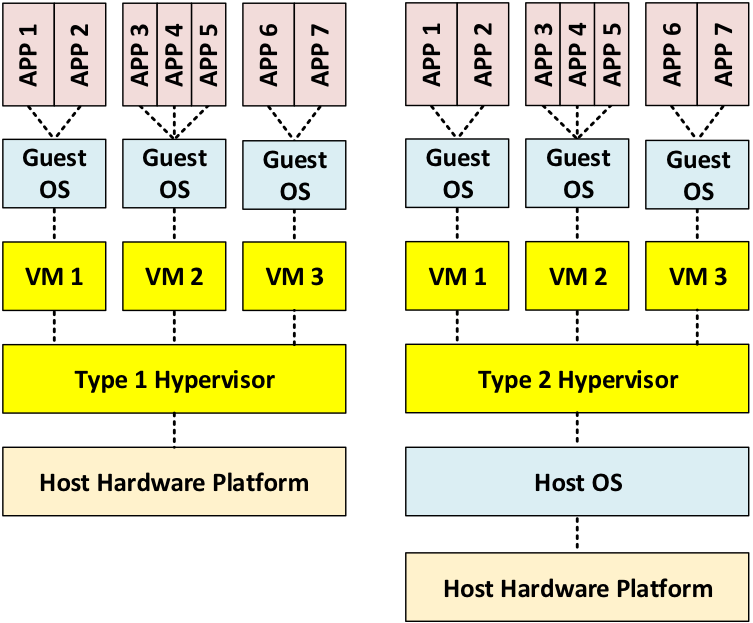
\includegraphics[width=8cm]{assets/virtualisation.png}
    \caption{Diagram illustrating how virtualisation works [5].}
    \label{fig:virtualisation}
  \end{figure}

  \subsection{Justification for a cloud-native approach}
  ACMEs' plan is an ambitious one, going from a paper-based system to a fully digitised solution that incorporates cryptocurrency are opposites! A large 
  factor is ACME's lack of starting infrastructure. The purchasing of servers, database and account management software alone would
  cost a lot of money. This financial burden is somewhat lessened by using a cloud-native approach as you pay for what you use and companies such as AWS offer
  a free tier [6].
  
  This type of architecture also enables the use of the sub-architectures like microservices which describe a \textit{'single application [that] is 
  composed of many loosely coupled and independently deployable smaller components' [7]}.

  \begin{figure}[H]
    \centering
    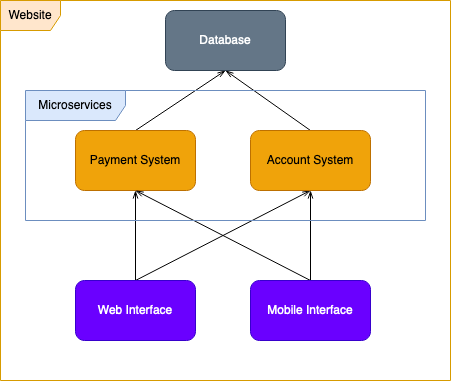
\includegraphics[width=8cm]{assets/microservices.drawio.png}
    \caption{Simple diagram illustrating how a system can use microservices.}
    \label{fig:microservices}
  \end{figure}

  Customers will go to competitors if they deem your service to be unreliable or cannot access you're system. Redundancy is provided by what AWS calls 
  AZs (Availability Zones) [8] these represent different data centers. So if one data center has an issue, your entire infrastructure can be \textit{'ported'} 
  to another one automatically. Coupled with this is the fact the services offered by these cloud providers have been tested by millions of people, so are 
  resilient, but also the cost to develop some of these solutions from scratch would be extremely costly.

  Using cloud-native providers also alleviates some of the responsibility. Google [9], AWS [10] and Azure [11] all have shared responsibility models where 
  they determine who oversees what. This gives a team less to worry about, as with certain packages operating systems, networking and even 
  security patches can all be handled and managed by the cloud provider.

  Finally a cloud-native approach is much more scalable and resilient. There are two ways to scale, vertically and horizontally.
  Vertically refers to adding more computing power, horizontally refers to adding extra machines [12].

  \begin{figure}[H]
    \centering
    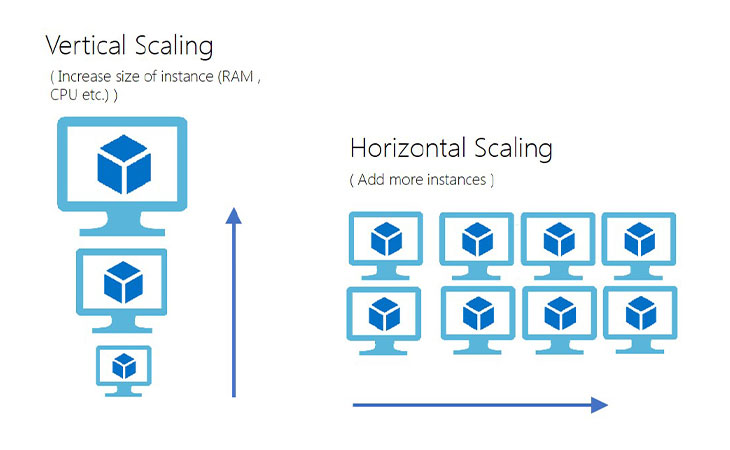
\includegraphics[width=8cm]{assets/scalingOptions.jpg}
    \caption{Diagram illustrating the different ways to scale infrastructure. [13]}
    \label{fig:scalingOptions}
  \end{figure}

  In an on-prem situation, scaling is expensive in both ways, buying a whole new server is not feasible for ACME, never mind the management of how
  redundancy takes place. But upgrading the hardware would also not be too cheap either. Cloud providers work at such a large scale that they can offer
  these features at a fraction of the cost that on-prem can. In addition there are options provided by the cloud providers to have fallbacks for failures and 
  load balancing for quicker response times. These are features that are costly to develop and maintain on ones own. 

  \subsection{Drawbacks of a cloud-native approach}
  Although there is a lot of positives to cloud-native, there is never a perfect solution. Here is a list of things to consider when adopting a cloud-native
  approach.

  \begin{itemize}
    \item \textbf{External dependency} - Adding another external dependency to a business is another thing that can go wrong. This year the BBC, Boots and
    others were caught up in an attack that revealed sensitive information about staff [14]. This was done by an attack using an external provider to gain 
    access to the companies using it. Although this is very unlikely, and even with full-control hacks could happen, it's something to consider.
    \item \textbf{Lock in} - Once you've picked a cloud provider to go with, the more infrastructure you build the harder it is to move away. With 
    IaC (Infrastructure as Code) [15] being used in a lot of organisations, it's not just a service switch, it can be the rewriting of 1000s of lines
    of code. Research is vital here, making sure the organisation you go with has the things you need and is expanding is vital to not reach a situation where
    you can't build what you want. 
    \item \textbf{Lack of control} - They could deprecate systems you were using leaving  you with a lot of issues. This has happened in the past with 
    certain version of software, for example node versions being deprecated [16]. The main reason this happens however is because the software is no 
    longer supported by the developers. This could lead to security issues in the future and it is therefore unsafe to use it. In addition to this, features 
    are usually \textit{soft deprecated} which refer to \textit{'an API which should no longer be used to write new code, but it remains safe to continue using 
    it in existing code'} [17].
    \item \textbf{Knowledge} - Cloud development and IAC [15] requires knowledge of how they work and piece together. ACME can put their developers who create
    the site on courses to learn this or hire a specialist who knows all about it already. This is an additional cost/factor to think about. I 
    don't see this is an issue though, as with the on-prem alternative you also need someone to manage the physical hardware as well as the software 
    running on it.
  \end{itemize}

  Despite these potentialities the realities; speed of development, fallbacks, lower cost and an array of services still make cloud-native the best choice.

  \newpage
  \subsubsection{Sub architectures in a cloud-native approach}
  As previously mentioned, using a cloud-native approach allows access to multiple services. These services have different architectures that we can take
  advantage of for individual parts/components of the system. Below breaks down the previous architecture into these separate architectures/services.

  \begin{figure}[H]
    \centering
    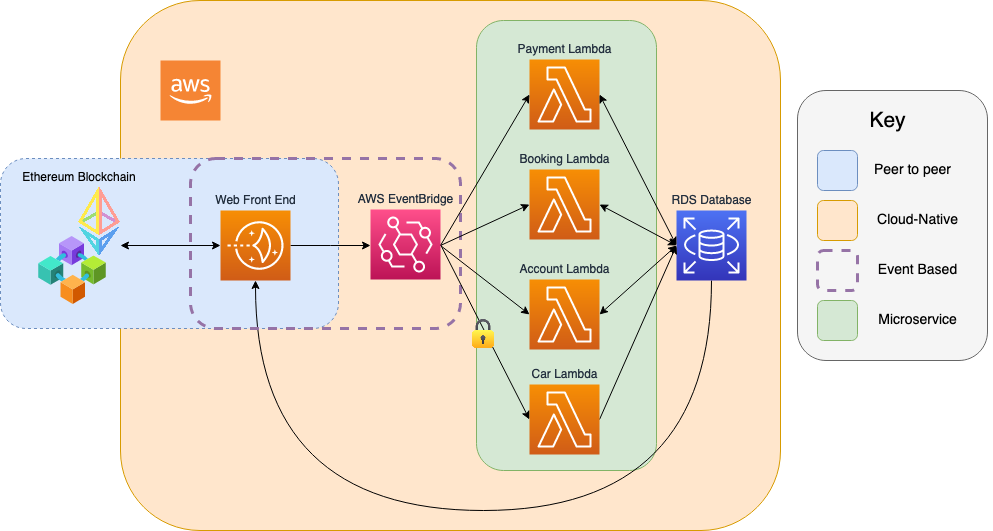
\includegraphics[width=12cm]{assets/architectureSectionedEvents.drawio.png}
    \caption{Diagram showing the proposed architecture with the different types of architecture labelled.}
    \label{fig:architectureSectioned}
  \end{figure}

  \begin{itemize}
    \item \textbf{Cloud-Native} - Cloud-native is the main architecture and \textit{'wraps'} around all the other architectures for the project. The benefits
    of this architecture have been discussed through this report.

    \item \textbf{Microservices} - Microservices have been mentioned in this report already, however the design illustrates how helpful they can be. The 4 
    lambdas in the design work independently of each other. If there's an issue with the payment lambda, users can still access the functionality provided by 
    the account lambda. Breaking the structure down this way also makes code more maintainable, as you can have separate repos for each component. A study 
    in 2017 [18] that compared 3 different deployment options, monolithic, microservices and lambda. In this study the microservices architecture still used
    EC2s/servers but instead had multiple smaller ones doing tasks, ACMEs' new design is more reminiscent of the \textit{'lambda'} implementation, which used
    different AWS services to achieve its goal. As can be seen in the below, the suggested architecture can not only be cheaper using the microservice/lambda 
    approach, but can actually result in quicker response times for the consumer.
    
    \begin{figure}[H]
      \centering
      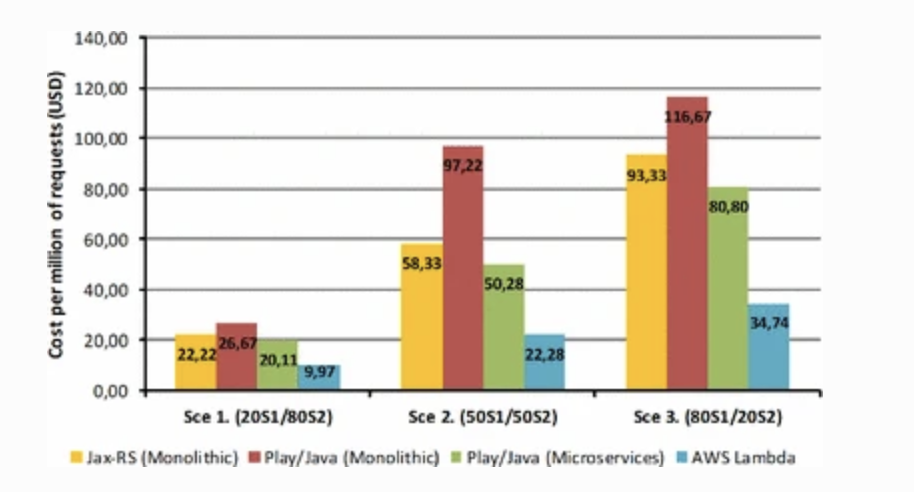
\includegraphics[width=8cm]{assets/costComparison.png}
      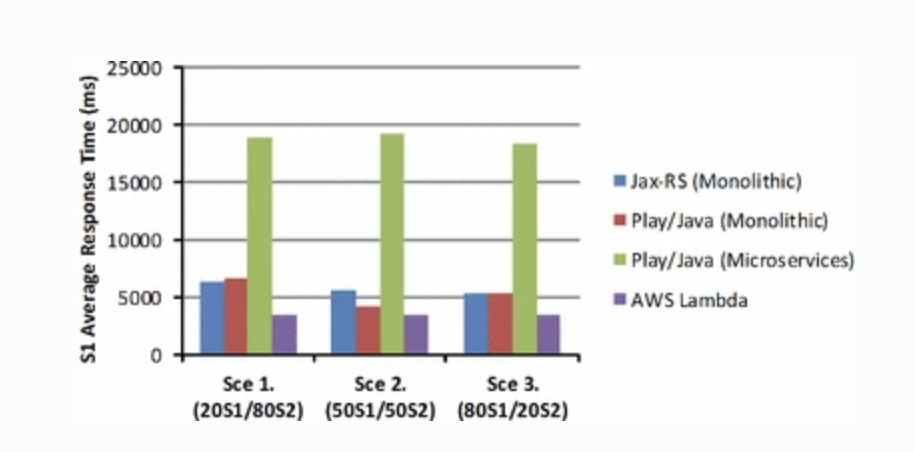
\includegraphics[width=8cm]{assets/responseTimeComparison.png}
      \caption{Charts showing results for the 3 solutions [19].}
      \label{fig:costComparison}
    \end{figure}

    Microservices aren't always the way to go, in fact Amazon themselves swapped away from this architecture for their live audio/video monitoring service [19].
    This makes sens as serverless/microservices are not made for continuous running. The microservices in ACMEs design would only run when they received events
    to do so.

    \item \textbf{Event-Based} - In the above design AWS EventBridge [19] is used to fire events to the individual lambdas. A benefit of this is the 
    responsiveness of the system. The client side has 0 wait time, as the event is fired off to the EventBridge which then routes the message to the correct 
    processor. Website performance is key to customer retention, one of ACMEs' business goals. An article by The Drum states that \textit{'79\% of people 
    wouldn't return to a site that had previously performed poorly for them' [20]}. Another article quotes:
    \begin{quote}
      \textit{'Previous research has shown that user frustration increases when page load times exceed eight to 10 seconds, without feedback' [21]}
    \end{quote}
    This event-driven approach minimises this load time. The EventBridge and its rules also filters out any bad traffic/events people try to send to it
    resulting in only valid event being processed.

    Some issues with event-based systems is error handling, which I will cover later in the report, and duplicated events. The system would have to have 
    some code built into it to stop people creating multiple orders instead of just the 1. Techniques like debouncing (\textit {'a function ensures that 
    it doesn't get called too frequently.'} [22]) can be used to stop this. 

    \item \textbf{Peer-2-Peer} - Finally my system is exposed to the P2P architecture due to the nature of cryptocurrency. Peer to peer can be described as:
    \begin{quote}
      \textit{'a decentralized platform whereby two individuals interact directly with each other, without intermediation 
      by a third party.'} [23]
    \end{quote}

    So if a user was to pay with cryptocurrency, there is no Stripe or bank in between ACME and their finances, ACME hs full control over that transaction.
    Smart contracts [24] can be used to automate and validate payments made, however this requires knowledge of the Solidity [25] programming language. 
    
    In my previous report I spoke about how quickly cryptocurrency adoption is growing. The automation through smart contracts allow and no middle-men 
    make the process easy to implement. Security of these contracts is paramount, so audits of this code should be carried out. Tools such as Chat GPT have been 
    tested to audit smart contracts, with mixed results [26][27].

  \end{itemize}

\newpage